\pagestyle{azougue}
\label{azougue}


\begin{textblock*}{5.625in}(0pt,0pt)%
\vspace*{-2.35cm}
\hspace*{-1.65cm}\includegraphics*[width=160mm]{./imgs/AZOUGUE.pdf}
\end{textblock*}

\pagebreak

%\hspace{.5cm}
%
%\begin{center}
%\hspace*{-.5cm}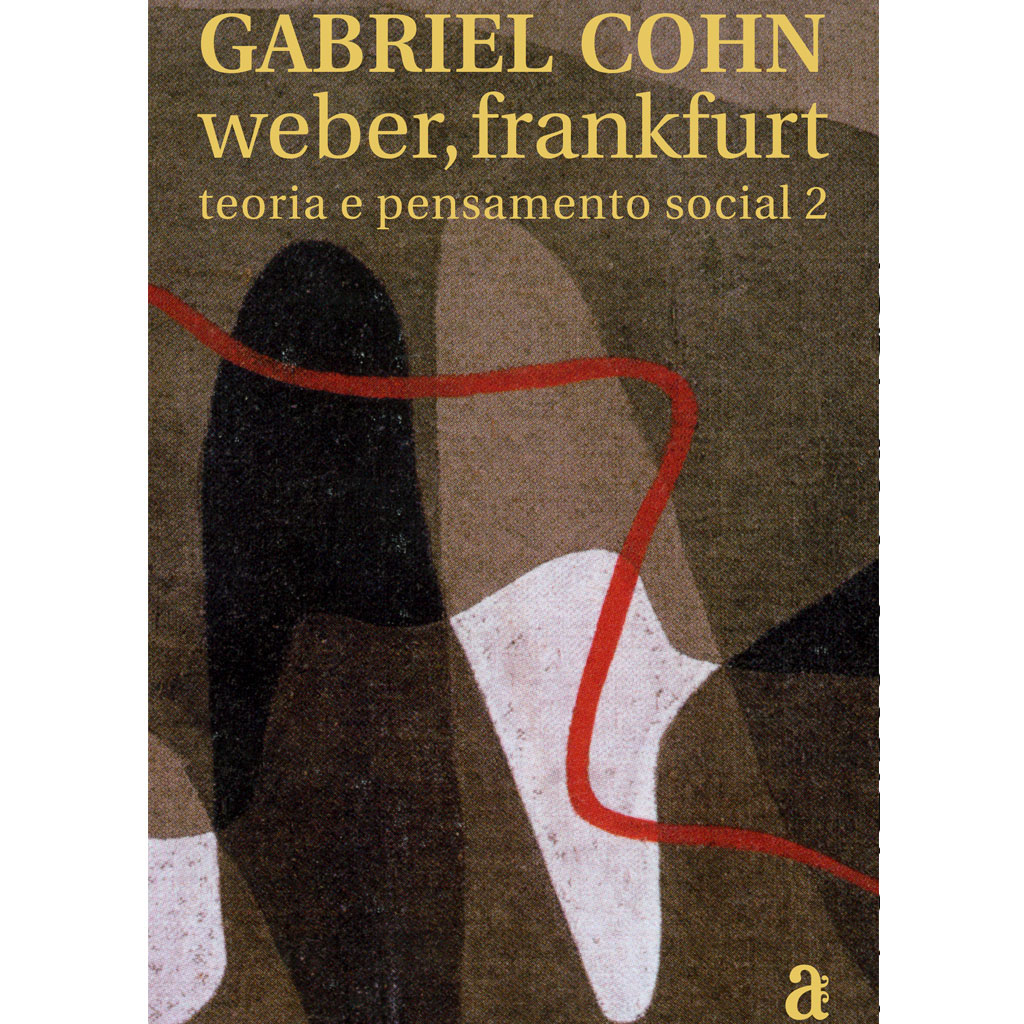
\includegraphics[width=45.5mm]{./imgs/weber.jpg}
%\end{center}
%
%\hspace*{-7cm}\hrulefill\hspace*{-7cm}
%
%\medskip
%
%\noindent{}Coletânea de textos sobre questões sociológicas, políticas e culturais, escritos nas últimas décadas pelo sociólogo, cientista político e professor emérito da \scalebox{.8}{USP} Gabriel Cohn. Traz estudos teóricos sobre pensadores internacionais de primeira linha, de Marx a Florestan Fernandes, passando por clássicos como Weber, Durkheim e autores da Escola de Frankfurt. Junta análises de problemas globais à realidade %brasileira, sobre questões fundamentais como as do desenvolvimento e da civilização.
%
%%\hspace{.5cm}
%\vfill
%
%\hspace*{-.4cm}\begin{minipage}[c]{1\linewidth}
%\small{
%{\Formular{\textbf{
%\hspace*{-.1cm}Título: Weber (Frankfurt 2)\\
%Autor: Gabriel Cohn\\ 
%Páginas: 268\\
%Formato: 17x24cm\\
%Preço: R\$ 54,90\\
%ISBN: 978-85-7920-235-3\\
%Disponibilidade: Em breve
%}}}}
%\end{minipage}
%
%\pagebreak

\hspace{.5cm}

\begin{center}
\hspace*{.5cm}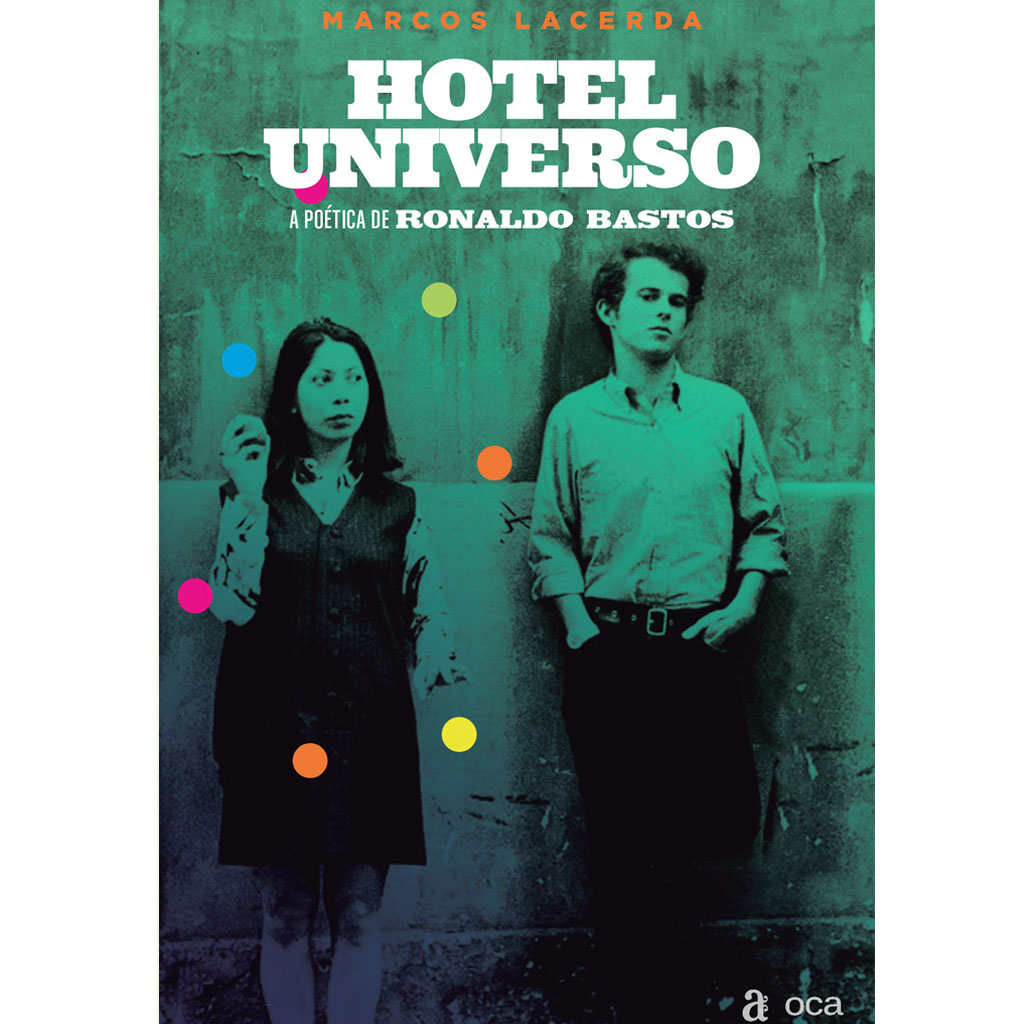
\includegraphics[width=92mm]{./grid/hotel.jpg}
\end{center}

\hspace*{-7cm}\hrulefill\hspace*{-7cm}

\medskip

\noindent{}{\slsc{Hotel Universo}} é uma antologia e análise profunda do cancioneiro e lírica de Ronaldo Bastos realizada por Marcos Lacerda, importante crítico musical da nova geração. Ronaldo Bastos é um dos principais compositores da canção brasileira: consegue estar ao mesmo tempo no centro da tradição mais sofisticada e inventiva da canção brasileira e ser também uma espécie de estrangeiro para esta mesma tradição. Foi um dos criadores e conceituadores mais destacados do Clube da Esquina, o movimento musical que revolucionou a poética e a estética da canção brasileira e teve como expoentes artistas do porte de Milton Nascimento, Beto Guedes e Lô Borges. Suas canções foram gravadas por nomes como Caetano Veloso, Elis Regina, Tom Jobim, Edu Lobo, Gal Costa, Maria Bethânia e Adriana Calcanhotto.

O autor Marcos Lacerda foi diretor de música da Funarte entre 2015 e 2017, responsável pela formulação, gestão e supervisão de políticas públicas de âmbito nacional. Organizou dois livros de ensaios sobre canção e música popular – mas aprofundou sua pesquisa sobre a obra de Bastos.

%\hspace{.5cm}
\vfill

\hspace*{-.4cm}\begin{minipage}[c]{.5\linewidth}
\small{
{\Formular{\textbf{
\hspace*{-.1cm}Título: Hotel Universo – a\\ poética de Ronaldo Bastos\\
Autor: Marcos Lacerda\\ 
ISBN: 978-85-7920-227-8\\
Páginas: 174\\
Formato: 14x21cm\\
Preço: R\$ 39,00\\
Editora: Azougue\\
Disponibilidade: Disponível
}}}}
\end{minipage}

\pagebreak

\hspace{.5cm}

\begin{center}
\hspace*{-2.5cm}\raisebox{6.8cm}{\rotatebox[origin=t]{90}{\huge\Formular{\textbf{Lançamento}}}}
\hspace*{2.5cm}
\includegraphics[width=92mm]{./grid/tembeta.jpg}
\end{center}

\hspace*{-7cm}\hrulefill\hspace*{-7cm}

\medskip

\noindent{}Grandes lideranças e pensadores indígenas estão reunidos em {\slsc{Tembetá}} --- do tupy, é o nome de um adorno usado no lábio inferior que simboliza o rito de passagem à maturidade. Primeiro volume de série voltada à cultura, educação, política, direitos humanos e ecologia que busca traçar o panorama plural do pensamento indígena contemporâneo através de entrevistas. A publicação busca tomar forma parecida, potencializando a voz dos povos originários em detrimento de uma fictícia e embolorada história dos “conquistadores”, num giro epistemológico a fim de entender a formação do Brasil e os caminhos possíveis para o futuro.

São seis quadros, feitos com Ailton Krenak, reconhecido internacionalmente como uma das maiores lideranças indígena, Álvaro Tukano, militante do movimento indígena e diretor do Memorial dos Povos Indígenas, Biraci Yawanawá, cacique da tribo Yawanawá, Eliane Potiguara, professora, escritora, ativista e fundadora da Rede Grumin de Mulheres Indígenas, Jaider Esbell e Sônia Guajajara, líder indígena e participante do Conselho de Direitos Humanos da \scalebox{.8}{ONU}.


%\hspace{.5cm}
\vfill

\hspace*{-.4cm}\begin{minipage}[c]{.5\linewidth}
\small{
{\Formular{\textbf{
\hspace*{-.1cm}Título: Tembetá\\
Autor: Sergio Cohn e Idjahure\\ Kadiwéu (org.)\\ 
ISBN: 978-85-7920-228-5\\
Páginas: 206\\
Formato: 14x21cm\\
Preço: R\$ 45,90\\
Editora: Azougue\\
Disponibilidade: Disponível
}}}}
\end{minipage}


\pagebreak

\hspace{.5cm}

\begin{center}
\hspace*{.5cm}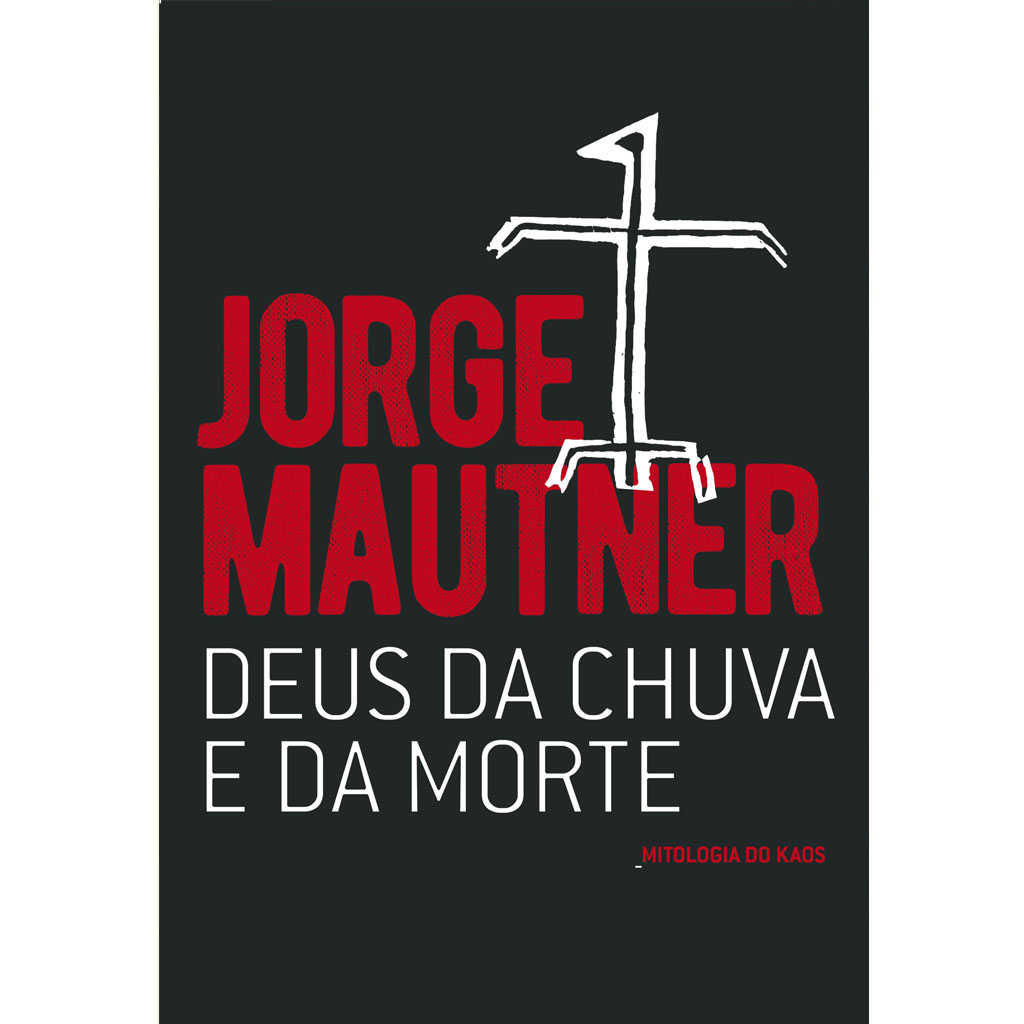
\includegraphics[width=92mm]{./grid/mautner.jpg}
\end{center}

\hspace*{-7cm}\hrulefill\hspace*{-7cm}

\medskip

\noindent{}Publicado em 1962, {\slsc{Deus da Chuva e da Morte}}, livro de estreia de Jorge Mautner, alcançou grande repercussão tanto de crítica como de público, conquistando o Prêmio Jabuti daquele ano e o consagrando como um dos autores mais singulares da literatura brasileira da época. Bebendo de inspirações do concretismo, da bossa"-nova e da literatura beatnik, o jovem Mautner, com apenas 19 anos, produziu literatura no mais alto nível. {\slsc{Deus da Chuva e da Morte}} trata de amor, música, tempo e revolução, em narrativa delirante que imprime ao texto sentimentos de toda uma geração revoltada e incompreendida.

Nas palavras de Caetano Veloso, que prefaciou a segunda edição do livro: “{\slsc{Deus da Chuva e da Morte}} tem a vitalidade das canções sentimentais e dos rocks que seu autor petulantemente exaltava contra todas as tendências de opinião da época. E tem a densidade do romantismo alemão. É, com tudo isso, uma obra de humor pop que fez os tropicalistas do final dos anos sessenta reconhecerem"-se ali profetizados. E não só os tropicalistas: a imaginação no poder, o sexo na política, a religião além da irreligião”.


%\hspace{.5cm}
\vfill

\hspace*{-.4cm}\begin{minipage}[c]{.5\linewidth}
\small{
{\Formular{\textbf{
\hspace*{-.1cm}Título: Mitologia do Kaos (Volume 1)\\
Autor: Jorge Mautner\\ 
ISBN: 978-85-7920-234-6\\
Páginas: 488\\
Formato: 16x23cm\\
Preço: R\$ 59,90\\
Editora: Azougue\\
Disponibilidade: Disponível
}}}}
\end{minipage}

\pagebreak

\hspace{.5cm}

\begin{center}
\hspace*{-2.5cm}\raisebox{6.8cm}{\rotatebox[origin=t]{90}{\huge\Formular{\textbf{Lançamento}}}}
\hspace*{2.5cm}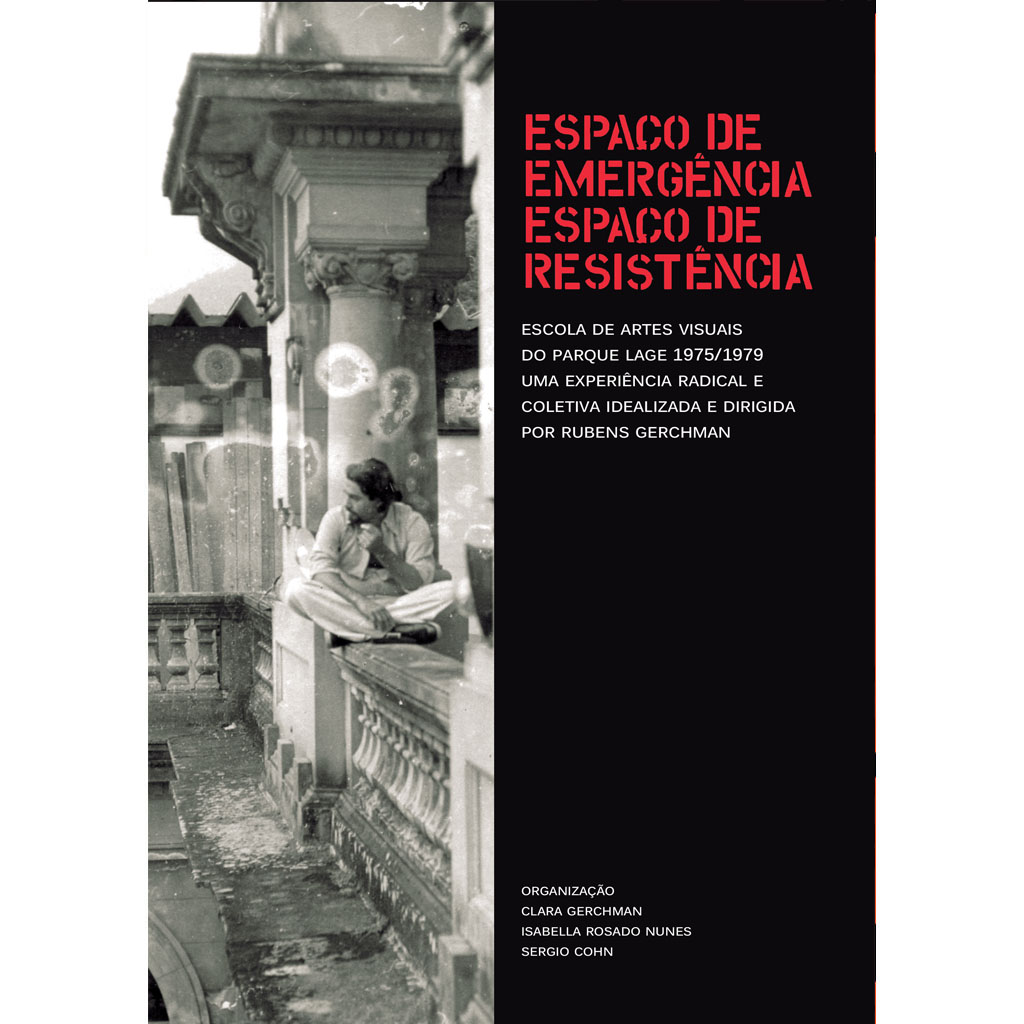
\includegraphics[width=92mm]{./grid/lage.jpg}
\end{center}

\hspace*{-7cm}\hrulefill\hspace*{-7cm}

\medskip

\noindent{}No final de 2008, o artista visual Rubens Gerchman gravou uma série de depoimentos sobre a criação e as experiências vivenciadas na Escola de Artes Visuais do Parque Lage (\scalebox{.8}{EAV}), que fundou e dirigiu entre agosto de 1975 e março de 1979. Ali se concretizava o que seria um de seus maiores desejos, manifestado em cartas, memórias e propostas de projetos: registrar e compartilhar a experiência coletiva de arte e educação da \scalebox{.8}{EAV}, desenvolvida em plena Ditadura Militar.

Este livro reúne as falas de Gerchman, além de documentos, cartas, recortes de jornal, material gráfico e uma série de 25 depoimentos com protagonistas da época, realizados por Clara Gerchman em parceria com os cineastas Bernardo Pinheiro e Pedro Rossi. Junto aos ensaios de Isabella Rosado Nunes, Suzana Velasco, Claudia Calirman e uma entrevista com Evandro Salles, permite um mergulho na \scalebox{.8}{EAV} da segunda metade da década de 70, um exercício experimental de liberdade no ensino e na vivência de arte no Brasil.


\vfill

\hspace*{-.4cm}\begin{minipage}[c]{.5\linewidth}
\small{
{\Formular{\textbf{
\hspace*{-.1cm}Título: Espaço de emergência,\\ espaço de resistência\\% — Escola de Artes Visuais do Parque Lage 1975-1979\\ %, uma experiência radical e coletiva idealizada e dirigida por Rubens Gerchman\\
Autor: Clara Gerchman, Isabella\\ Rosado Nunes e Sergio Cohn (org.)\\ 
ISBN: 978-85-7920-226-1\\
Páginas: 156\\
Formato: 14x21cm\\
Preço: R\$ 39,90\\
Editora: Azougue\\
Disponibilidade: Disponível
}}}}
\end{minipage}


\pagebreak
\pagestyle{azouguecat}

\begin{multicols}{2}
\begin{enumerate}
\setlength\parskip{8pt}
\setlength\itemsep{-1.4mm}
\item Encontros: Newton Da Costa, {\Formular{\textbf{Newton Da Costa}}}
\item Encontros: Maio de 68, {\Formular{\textbf{Maio de 68}}}
\item Encontros: Jomard Muniz de Britto, {\Formular{\textbf{Jomard Muniz de Britto}}}
\item Encontros: Gilberto Gil, {\Formular{\textbf{Gilberto Gil}}}
\item Encontros: Eduardo V. de Castro, {\Formular{\textbf{Castro, Eduardo V. de}}}
\item Encontros: Eduardo Coutinho, {\Formular{\textbf{Eduardo Coutinho}}}
\item Encontros: Darcy Ribeiro, {\Formular{\textbf{Darcy Ribeiro}}}
\item Encontros: Capoeira, {\Formular{\textbf{Capoeira}}}
\item Minima Moralia, {\Formular{\textbf{Theodor Adordo}}}
\item Ensaios fundamentais - cinema, {\Formular{\textbf{Sérgio Cohn}}}
\item A odisseia, {\Formular{\textbf{Flavio Basso; Julio Manzi}}}
\item Plano nacional de cultura, {\Formular{\textbf{Guilherme Varella}}}
\item Encontros: Nise Da Silveira, {\Formular{\textbf{Nise Da Silveira}}}
\item Encontros: Rogerio Sganzerla, {\Formular{\textbf{Rogerio Sganzerla}}}
\item Encontros: Jorge Mautner, {\Formular{\textbf{Jorge Mautner}}}
\item Encontros: Milton Santos, {\Formular{\textbf{Milton Santos}}}
\item Encontros: Vinicius de Moraes, {\Formular{\textbf{Vinicius de Moraes}}}
\item Encontros: Zé Celso Martinez Correa, {\Formular{\textbf{Zé Celso Martinez Correa}}}
\item Encontros: Ricardo Aleixo, {\Formular{\textbf{Ricardo Aleixo}}}
\item Encontros: Wanderley Guilherme, {\Formular{\textbf{Wanderley Guilherme}}}
\item Encontros: Luiz Rosemberg Filho, {\Formular{\textbf{Luiz Rosemberg Filho}}}
\item Encontros: Arnaldo Antunes, {\Formular{\textbf{Arnaldo Antunes}}}
\item Encontros: Flavio de Carvalho, {\Formular{\textbf{Flavio de Carvalho}}}
\item Encontros: Ailton Krenak, {\Formular{\textbf{Ailton Krenak}}}
\item Encontros: Gilberto Mendes, {\Formular{\textbf{Gilberto Mendes}}}
\item Encontros: Julio Cortazar, {\Formular{\textbf{Julio Cortazar}}}
\item Encontros: Aloisio Magalhães, {\Formular{\textbf{Aloisio Magalhães}}}
\item Encontros: Paulo Emilio Sales Gomes, {\Formular{\textbf{Paulo Emilio Sales Gomes}}}
\item Encontros: Mario Pedrosa, {\Formular{\textbf{Mario Pedrosa}}}
\item Encontros: Antonio Cicero, {\Formular{\textbf{Antonio Cicero}}}
\item Encontros: Nara Leão, {\Formular{\textbf{Nara Leão}}}
\item Encontros: Tropicália
\item Encontros: Dias Gomes, {\Formular{\textbf{Dias Gomes}}}
\item Encontros Carlos Drummond de Andrade, {\Formular{\textbf{Carlos Drummond de Andrade}}}
\item Encontros Clarice Lispector, {\Formular{\textbf{Clarice Lispector}}}
\item Encontros: Sergio Buarque de Holanda, {\Formular{\textbf{Sergio Buarque de Holanda}}}
\item Encontros: Tom Jobim, {\Formular{\textbf{Tom Jobim}}}
\item Encontros: Tom Zé, {\Formular{\textbf{Tom Zé}}}
\item Encontros: Mario Schenberg, {\Formular{\textbf{Mario Schenberg}}}
\item Encontros: Geração Beat, {\Formular{\textbf{Geração Beat}}}
\item Encontros: Lucio Costa, {\Formular{\textbf{Lucio Costa}}}
\item Encontros: Manoel de Barros, {\Formular{\textbf{Manoel de Barros}}}
\item Encontros: Boris Schnaiderman, {\Formular{\textbf{Boris Schnaiderman}}}
\item Encontros: Silviano Santiago, {\Formular{\textbf{Silviano Santiago}}}
\item Encontros: Roberto Piva, {\Formular{\textbf{Roberto Piva}}}
\item Encontros: Helio Oiticica, {\Formular{\textbf{Helio Oiticica}}}
\item Encontros: Antonio Riserio, {\Formular{\textbf{Antonio Riserio}}}
\item Encontros: Paulo Freire, {\Formular{\textbf{Paulo Freire}}}
\item Encontros: Paulo Mendes Da Rocha, {\Formular{\textbf{Paulo Mendes Da Rocha}}}
\end{enumerate}
\end{multicols}

\pagebreak
